\begin{savequote}[8cm]
%Well, think. When do light and electrons and nuclei behave like a particle - like a quantum? When they bump into anything, right? When they hit a wall - that sort of thing. 
%  \qauthor{--- Russell Stannard's \textit{Uncle Albert}}
Ok, everyone back to the lab, try again.
   \qauthor{--- MF DOOM, \textit{Books of War}}
\end{savequote}

\chapter{\label{ch:4-effmass}Electronic band non-parabolicity}

\section{Introduction}
%% Need to include references to the three appendices.

Many semiconductor properties depend on the response of electrons to an external pertubation.
This perturbation could take the form of an electric field, change in temperature or an applied lattice stress.  %what else??
In a crystal, this response depends on the interaction of the electrons with a periodic potential. 
The effective mass approximation assumes that the response of an electron in a periodic potential is equivalent to that of a free electron with a renormalised mass (called the ``effective mass'').
This makes the effective mass a critical parameter in models for the optical and transport properties of a semiconductor.
Recently there has been renewed interest in this research area, in particular the impact of electronic bandstructure anisotropy and non-parabolicity on the properties of thermoelectric materials.\autocite{Gibbs2017,Mecholsky2014}

The conventional definition of effective mass is
\begin{equation} \label{curvature}
\frac{1}{m_\text{c}}= \frac{1}{\hbar^2}\frac{\partial^2E}{\partial k^2}.
\end{equation}
This is derived using Newton's second law\autocite{Ashcroft1976,Ariel2012} and so is commonly referred to as the inertial effective mass or conductivity effective mass (as it describes the acceleration of an electron in an applied electric field).
In principle, this allows effective masses to be calculated directly from \textit{ab-initio} bandstructures,
as $m_\text{c}$ is inversely proportional to the curvature of the electronic dispersion in reciprocal space (Figure\ \ref{effmass_schematic}). 
We will refer to this definition as the curvature effective mass.

For semiconductor materials with a low carrier concentration we are often interested in eigenstates close to the band extrema where the dispersion can be approximated with an isotropic parabola

\begin{equation} \label{parabolic}
E(k)= \frac{\hbar^2k^2}{2m^*}.
\end{equation}

This approximation leads to an effective mass which is independant of the sampling density and range in reciprocal space.
However, non-parabolic deviations in the true dispersion mean that the effective mass obtained from a particular bandstructure depends on the approach used to numerically calculate Eqn.\ \ref{curvature}. 

At greater carrier concentrations and higher temperatures, higher energy eigenstates are accessed and it becomes increasingly important to account for band non-parabolicity.\autocite{Ruf1990} 
To describe a non-parabolic band dispersion we keep the second order $k^2$ ellipsoidal energy surfaces and introduce a non-linear dependence on the energy, 
\begin{equation} \label{nonparabolic}
\frac{\hbar^2k^2}{2m^*} = \gamma(E) = E + \alpha E^2 + \beta E^3+ \ldots .
\end{equation}

Keeping the first non-linear term gives the Kane quasi-linear dispersion relation\autocite{Kane1957}

\begin{equation} \label{kane}
\frac{\hbar^2k^2}{2m^*} = E(1 + \alpha E),
\end{equation}

where $\alpha$ is a parameter that quantifies the extent of non-parabolicity; for the perfectly parabolic material this would be equal to zero. 
$\alpha$ is positive for electrons in the conduction band (CB) and negative for electrons in the valence band (VB). 
This corresponds to a flattening of the band as the difference between the eigenstate energy and the band edge energy is increased (Figure\ \ref{dispersion_fits}).

\begin{figure}[tb] \centering
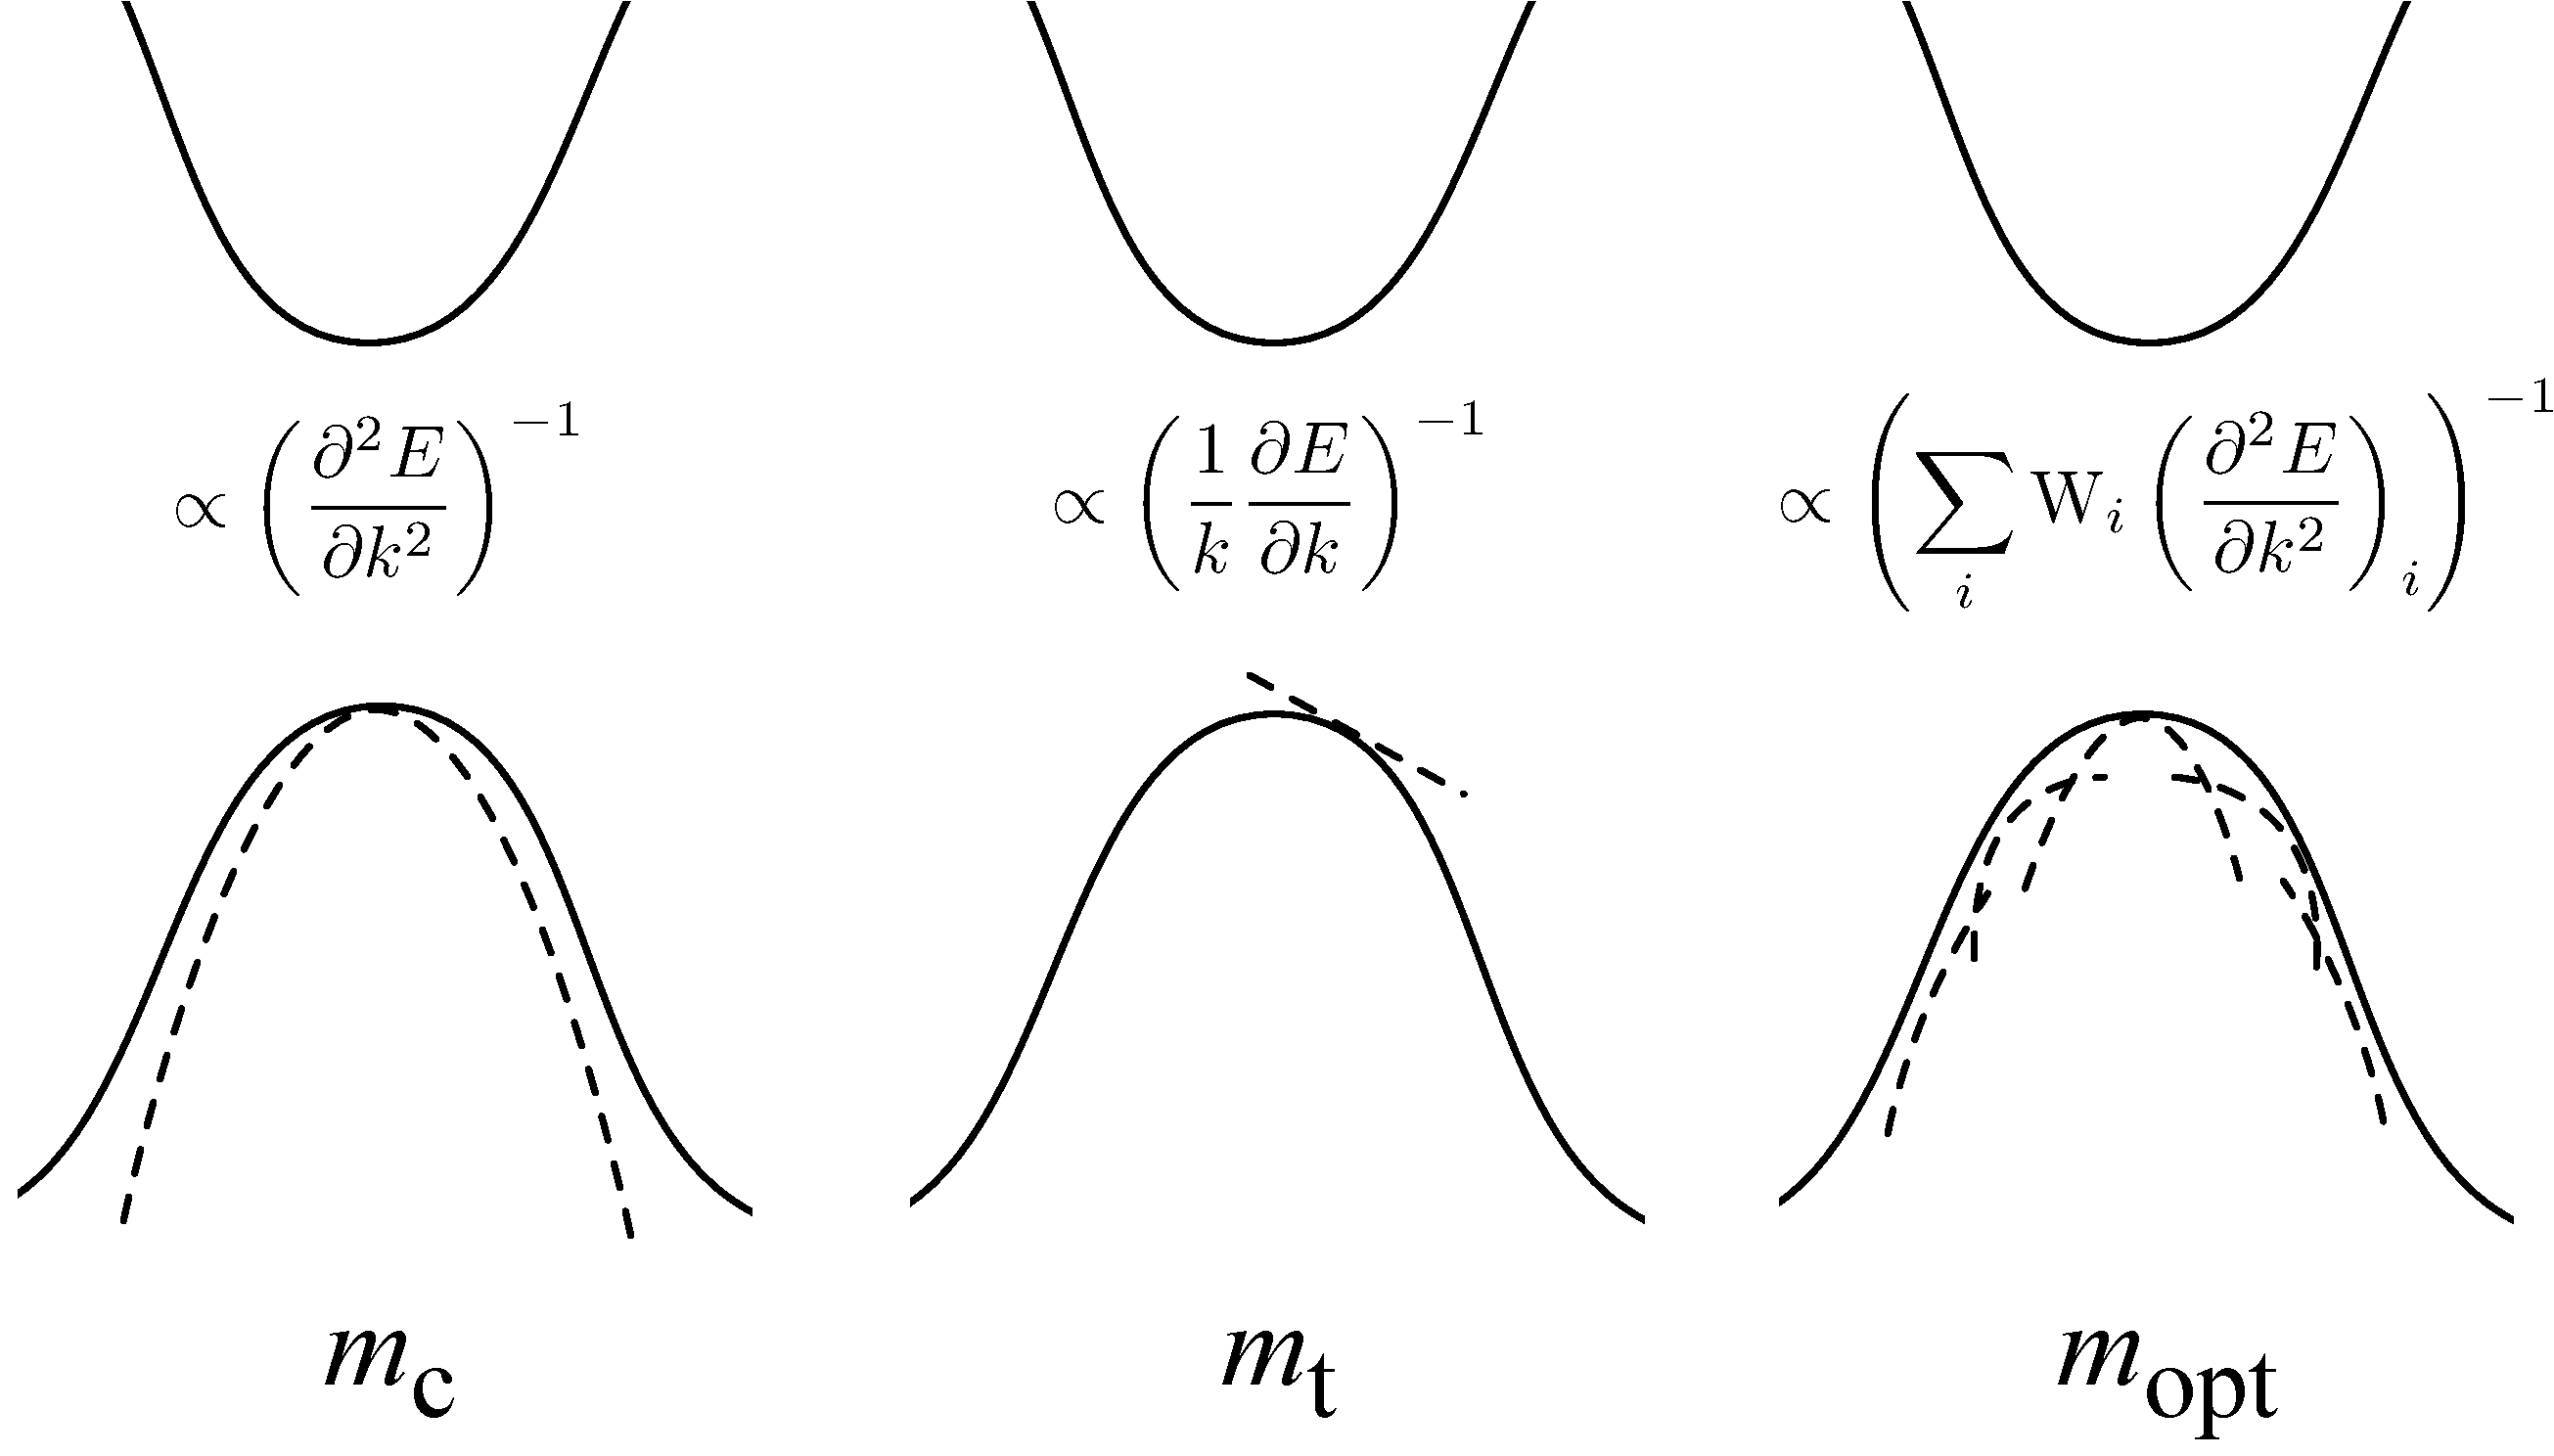
\includegraphics[width=0.6\textwidth]{./figures/ch4/effmass_schematic.pdf}
\caption[Schematic of the three definitions for effective mass]{\label{effmass_schematic} The three definitions for effective mass used in this chapter are: i) the curvature effective mass $m_{\text{c}}$, which is inversely proportional to the curvature of the electronic dispersion in reciprocal space; ii) the optical effective mass $m_{\text{opt}}$, which is the average curvature effective mass, weighted according to the Fermi--Dirac distribtion; and iii) the transport effective mass $m_{\text{t}}$. }
\end{figure}

For non-parabolic dispersions we use the following definition of effective mass
\begin{equation} \label{transport}
\frac{1}{m_\text{t}} = \frac{1}{\hbar^2 k}\frac{\partial E}{\partial k}.
\end{equation}
This is the mass which relates the momentum and velocity of an electron wavepacket in the equation $mv = \hbar k$,\autocite{Ariel2012} thus it is often referred to as the transport effective mass.
For parabolic dispersions, it is equal to the curvature effective mass given in Eqn.\ \ref{curvature}. 
For the Kane quasi-linear dispersion, the transport effective mass is given by
\begin{equation} \label{kanemass}
m_\text{t}(E) = m_0(1+2 \alpha E),
\end{equation}
where $m_{0}$ is the transport effective mass at the band edge.\autocite{Segev2005} 
By using the Kane dispersion as a more accurate approximation to the real material dispersion, the effective mass becomes linearly dependant on the particle energy.
As a result, the effective mass will increase as we fill the band with charge carriers through doping, photo-excitation or an increase in temperature.\autocite{Riffe2002}
Material properties which are dependant on effective mass, such as electron and hole mobility, will also change as the carrier concentration is increased.
This is in contrast to the parabolic approximation which leads to a constant effective mass that is independant of energy.

There are multiple definitions for effective mass, each valid according to the perturbation which is under consideration.
To calculate an effective mass which is comparable to that measured in optical experiments we use the definition for optical effective mass

\begin{equation}
\frac{1}{m_{\text{opt}}} = \frac{2}{n_{\text{e}}}\sum_{\text{l}}\sum_{\text{k}}^{\text{occ}} \frac{1}{m_\text{c}^{\text{l}}(k)},
\end{equation}
where $m_{\text{c}}^{\text{l}}$ is the curvature effective mass for band $\text{l}$ and $n_{\text{e}}$ is the carrier concentration. 
The summation over all occupied eigenstates $k$ of each band l accounts for any non-parabolicity. 
This definition has been used in the context of thermoelectric materials\autocite{Gibbs2017} and transparent conducting oxides.\autocite{Hautier2013} 

Using Fermi--Dirac statistics, and following a derivation from Huy \textit{et al.},\autocite{Huy2011} we can replace the summation over occupied states with an integral along one-dimensional slices of reciprocal space
\begin{equation} \label{opt2}
\frac{1}{m_{\text{opt}}} = \frac{\displaystyle\sum_{\text{l}} \displaystyle\int f(E,T) \frac{\partial^2 E}{\partial k^2} dk}{\displaystyle\sum_{\text{l}} \displaystyle\int f(E,T) dk},
\end{equation}
where $f(E,T)$ is the Fermi--Dirac distribution for particle at energy $E$ and system at temperature $T$
\begin{equation} \label{fermidirac}
f(E,T) = \frac{1}{\exp\left(\frac{E-E_{\text{F}}}{k_{\text{B}}T}\right)+1}.
\end{equation}

In the case of one occupied branch at $T=0\,\mathrm{K}$ we reach the transport effective mass evaluated at the Fermi level
\begin{equation} \label{opt}   
\frac{1}{m_{\text{opt}}} = \cfrac{\displaystyle\int_0^{k} \cfrac{1}{\hbar^2}\frac{\partial^2E}{\partial k^2} dk}{\displaystyle\int_0^{k}dk} = \frac{1}{\hbar^2k_{\text{F}}} \frac{\partial E}{\partial k}\biggr\rvert_{k=k_{\text{F}}},
\end{equation}
where $k_{\text{F}}$ is the Fermi wavevector.

The extent to which this value of effective mass will increase as the carrier concentration increases depends on the extent of band non-parabolicity and the level to which the bands are filled. 
The level of band-filling can be measured experimentally via the Burstein--Moss band gap shift.\autocite{Burstein1954,Moss1954} 
This is a concentration-dependant shift in the absorption edge which was used for the characterisation of \ce{GaAs} and other small bandgap semiconductors in the 1970's. 

\begin{figure}[tb] \centering
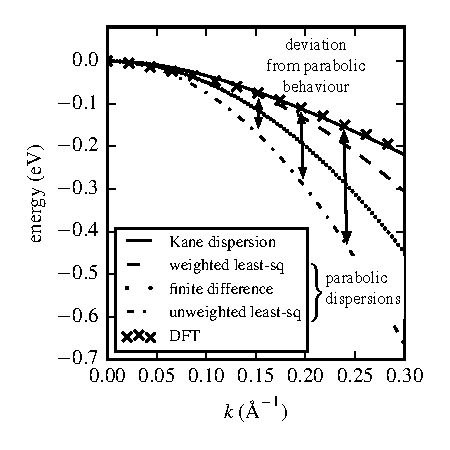
\includegraphics[width=0.6\textwidth]{./figures/ch4/fits_to_dispersion.pdf}
\caption[Numerical methods for fitting a band dispersion]{\label{dispersion_fits} The electronic valence band dispersion in the [110] direction of \ce{Cu2ZnSnS4}. The DFT dispersion is non-parabolic away from the band edge with $\alpha$, the Kane dispersion parameter, equal to ${2.2}$. The curvature effective mass depends upon the numerical method used, as shown by the three different parabolas (dash, dot and dash-dot lines). At higher binding energies the Kane quasi-linear dispersion (continuous line) gives a better approximation to the DFT dispersion. Calculations use the hybrid exchange-correlation functional HSE06 with spin-orbit coupling.}
\end{figure}

Transient absortion spectroscopy can be used to measure the Burstein--Moss band gap shift, from which the effective mass and shape (parabolicity) of the electronic bands can be inferred.
Three studies have calculated the Burstein--Moss shift in the hybrid halide perovskite \ce{CH3NH3PbI3} (MAPI), with values for the effective mass ranging from $0.14\,m_{\text{e}}$--$0.30\,m_{\text{e}}$ (where $m_{\text{e}}$ is the electron rest mass).\autocite{Manser2014,Yang2015,Price2015}
Although each model differs in detail (Yang \textit{et al.} consider band gap renormalisation,\autocite{Yang2015} whilst Price \textit{et al.} consider photoinduced refractive index changes\autocite{Price2015}), none of the models account for bandstructure non-parabolicity, despite previous computational studies which report significant non-parabolicity in MAPI within an energy range accesible at room temperature ($k_\mathrm{B}T=25\,\mathrm{meV}$ at $T=300\,\mathrm{K}$). 

As outlined previously, for any dispersion that is not parabolic, the calculated effective mass will depend upon the numerical method used to calculate band curvature and carrier concentration.
For materials with a significant number of excited carriers, the discrepancy between the parabolic and non-parabolic effective mass can be large.\autocite{Ruf1990,Riffe2002}
An \textit{ab-intio} effective mass which recognises the non-parabolicity of real materials allows for better prediction of important material properties such as carrier mobility. 

In this chapter I calculate the curvature effective mass and $\alpha$ parameter of four photovoltaic materials: \ce{CdTe}, \ce{GaAs}, \ce{MAPI} and \ce{CZTS}. 
First I consider how sensitive the effective mass is to the method and sampling density used to calculate the band curvature. 
For this, the results obtained using three different methods are compared. 
Two of these are widely used to calculate the curvature effective mass: a three-point finite difference and a least-squares quadratic fit. 
The third method is a new approach which uses a least-squares quadratic fit weighted according to Fermi--Dirac statistics. 
The results at different levels of theory are then compared to assess the impact of spin-orbit coupling and electron exchange-correlation on the calculated values for effective mass and $\alpha$. 
Finally, the effect of non-parabolicity on the optical and transport properties of MAPI at high carrier concentrations is considered. 
It is shown that the Burstein--Moss shift is severely overestimated if calculated within the parabolic approximation, and that the Kane quasi-linear dispersion leads to accurate predictions.
The optical effective mass and electron mobility is predicted, over a carrier concentration range of $10^{16}$--$10^{20}\,\mathrm{cm}^{-3}$, which is the relevant range for concentrated solar power systems ($\sim10^{18}\,\mathrm{cm}^{-3}$)\autocite{Law2014}, or when excited under a laser for transient absorption or photoluminescence studies ($\sim10^{19}\,\mathrm{cm}^{-3}$).
It is found that non-parabolicity leads to a significant change in transport properties for carrier concentrations above $10^{18}\,\mathrm{cm}^{-3}$.


\section{Methods} \label{ch4:methods}

\subsection{Calculation procedures for effective mass}

One-dimensional slices through the Brillouin zone are considered so that the effective mass tensor is reduced to a function of one variable $k$. Unless otherwise stated, the Fermi--Dirac distribution is calculated at $T=300\,\mathrm{K}$ with the Fermi level set in the middle of the bandgap.

\subsubsection{Curvature effective mass at the band edge}

Three approaches are used to calculate the curvature effective mass at the band edge: i) a three point forward finite difference method; ii) an unweighted quadratic least-squares fit\autocite{Vanderwalt2011} to three points; iii) a quadratic least-squares fit, weighted according to the Fermi--Dirac distribution across all points up to energy $10\,\mathrm{k_\mathrm{B}T}$ ($=0.25\,\mathrm{eV}$).

\textit{Finite difference:} \\
A three point forward finite difference equation is used to calculate the curvature at point $i$:

\begin{equation}
\frac{\partial^2E}{\partial k^2} = \frac{E_{i+2} - 2E_{i+1} + E_i}{\left|k_{i+1} - k_i\right|},
\end{equation}
where $E_\mathrm{i}$ is the energy eigenvalue at position $k_\mathrm{i}$ in reciprocal space. 

\textit{Unweighted least-squares fit:}\\
To obtain an estimate for the coefficient $c$ of a parabolic dispersion

\begin{equation}
E = {c}k^2,
\end{equation}
A least-squares method as implemented in the \textsc{NumPy} Python library is used to minimise the summed square of residuals

\begin{equation}
\sum^{5}_{i=1}(\mathrm{c}k_{i}^2 - E_{i})^2.
\end{equation}
This is a five point fit; three points from the DFT-calculated dispersion plus two from the symmetry of the dispersion ($E(k)=E(-k)$).

\textit{Weighted least-squares fit:}\\
To obtain an estimate for the coefficient $c$ of a parabolic dispersion

\begin{equation}
E = \mathrm{c}k^2,
\end{equation}
A weighted least-squares method is used as implemented in the \textsc{NumPy} Python library to minimise the summed square of residuals

\begin{equation}
\sum^n_{i=1}W_i(\mathrm{c}k_i^2 - E_i)^2.
\end{equation}
The summation is over all points up to an energy of $0.25\,\mathrm{eV}$, including points generated from the symmetry of the dispersion ($E(k)=E(-k)$). 
$W_i$ is given by

\begin{equation}
W_{i}(E_i,T=300\,\mathrm{K}) = \frac{1}{\exp\left(\frac{E_i-E_{\text{f}}}{k_{\text{B}}T}\right)+1}.
\end{equation}

Due to the exponential term in $W_i$, points with an energy difference larger than $0.25\,\mathrm{eV}$ contribute a negligible amount to the weighted sum. 

\subsubsection{Kane dispersion parameters}

To calculate the parameters for the Kane dispersion a sixth order polynomial is fitted to the DFT calculated electronic band dispersion over an energy range of $0.25\,\mathrm{eV}$. The first derivative of this continuous function is used to determine the transport effective mass. The transport effective mass is plotted against energy to give values for $\alpha$ and the effective mass at the band edge. The dispersion is truncated where the second derivative changes sign as this corresponds to an inflexion point where the Kane dispersion is no longer valid. 
%The alpha values in table \ref{largetable} were calculated from a Kane dispersion fitted over an energy range of minimum 0.09eV.

\subsubsection{Optical effective mass}

To calculate the optical effective mass the integrand in Eqn.\ \ref{opt} is numerically integrated with $E(k)$ given by the Kane dispersion. Convergence with respect to energy is fast as the Fermi--Dirac distribution kills the probability of eigenstate occupation exponentially. 

\subsection{Electronic bandstructure calculations}

For each system, the atomic structures and calculated band dispersions were relaxed using density functional theory (DFT) as implemented in the Vienna \textit{Ab-initio} Simulation Package (\textsc{VASP}).\autocite{Kresse1996} The valence wavefunctions were expanded in a plane wave basis set with a cut-off of $500\,\mathrm{eV}$. Scalar-relativistic corrections for the core electrons were used within the projector augmented wave formalism.\autocite{Blochl1994}
The initial structure was determined as follows: Si and \ce{GaAs} structures were taken from the Madelung handbook,\autocite{Madelung2004}  \ce{CdTe}\autocite{Rabadanov2001} and \ce{CZTS}\autocite{Lafond2014} (in the tetragonal phase) were determined from X-ray diffraction data, whilst \ce{MAPI} was optimised starting from a pseudo-cubic (high temperature) structure available online.\autocite{WMD} For all relaxations a quasi-Newtonian algorithm and the PBEsol exchange-correlation functional were used.

For each calculation the Brillouin zone was sampled using a Monkhorst-Pack $\Gamma$-centred $k$-point mesh. For silicon, CdTe, GaAs and MAPI a $6\!\times\!6\!\times\!6$ grid was used. For CZTS, which has a tetragonal crystal structure, a $6\!\times\!6\!\times\!4$ grid was used. This was followed with a non-self-consistent calculation along high symmetry lines\autocite{Setyawan2010}, with points spaced $0.005\,\text{\AA}^{-1}$ apart in reciprocal space, except in the case of the hybrid HSE06 functional with spin-orbit coupling, where a spacing of $0.02\,\text{\AA}^{-1}$ was used. The total energy of each material was converged to within $10^{-6}\,\mathrm{eV}$. Exchange and correlation was modelled using: (i) the local density approximation (LDA); (ii) the PBEsol\autocite{Perdew2008} generalized gradient approximation, and (iii) the screened hybrid functional HSE06.\autocite{Heyd2003} Spin-orbit coupling (SoC) was used at the PBEsol and HSE06 levels of theory to investigate relativistic effects. A comparison between the bandstructures with and without SoC can be found in Appendix \ref{app:2-bandstructures}.
The density-of-states of MAPI was investigated using tetragonal smearing and the HSE06 functional with SoC. 

\begin{landscape}
\newcommand{\ra}[1]{\renewcommand{\arraystretch}{#1}}
\begin{table}[tb]\centering
\ra{1.3}
\begin{tabular}{@{}lclllclllclllclll@{}}\toprule
& \phantom{abc}&\multicolumn{3}{c}{finite diff $m_\text{c}\left(m_{\text{e}}\right)$} & \phantom{abc}& \multicolumn{3}{c}{unweighted $m_\text{c}\left(m_{\text{e}}\right)$} &\phantom{abc} & \multicolumn{3}{c}{weighted $m_\text{c}\left(m_{\text{e}}\right)$} & \phantom{abc} & \multicolumn{3}{c}{$\alpha \left(\mathrm{eV}^{-1}\right)$}\\
\cline{3-5} \cline{7-9} \cline{11-13} \cline{15-17}
&& [100] & [110] & [111]$^*$  && [100] & [110] & [111]$^*$   && [100] & [110] & [111]$^*$   && [100] & [110] & [111]$^*$  \\ 
\midrule
GaAs\\
light hole 
&& 0.09 & 0.08 & 0.05        &&  0.08    & 0.07  & 0.07     && 0.09 & 0.08 & 0.08     && 3.32 & 3.64 & 3.69  \\
heavy hole 
&& 0.37 & 0.73 & 0.79        &&  0.31    & 0.58  & 0.25     && 0.32 & 0.75 & 0.53     && 0.38 & 3.37 & 1.70  \\
electron 
&& 0.07 & 0.07 & 0.06        &&  0.06    & 0.06  & 0.06     && 0.06 & 0.07 & 0.07     && 1.05 & 1.15 & 1.23  \\
CdTe\\
light hole 
&& 0.11 & 0.10 & 0.10        &&  0.11    & 0.10  & 0.10     && 0.12 & 0.10 & 0.10     && 1.25 & 1.49 & 1.64  \\
heavy hole 
&& 0.45 & 0.86 & 1.09        &&  0.44    & 0.83  & 1.20     && 0.45 & 0.83 & 1.06     && 0.38 & 0.99 & 0.77  \\
electron 
&& 0.09 & 0.09 & 0.09        &&  0.09    & 0.09  & 0.09     && 0.09 & 0.10 & 0.10     && 0.72 & 0.94 & 1.02  \\
MAPI\\
hole 
&& 0.28 & 0.15 & 0.14        &&  0.15    & 0.09  & 0.12     && 0.23 & 0.10 & 0.12     && 4.27 & 1.88 & 1.32  \\
electron 
&& 0.15 & 0.13 & 0.12        &&  0.18    & 0.10  & 0.19     && 0.19 & 0.10 & 0.18     && 2.21 & 1.35 & 0.16  \\
CZTS\\
hole 
&& 0.23 & 0.74 & 0.75        &&  0.22    & 0.54  & 0.60     && 0.32 & 1.16 & 1.23     && 3.96 & 2.21 & 1.50  \\
electron 
&& 0.19 & 0.19 & 0.19        &&  0.18    & 0.18  & 0.18     && 0.19 & 0.19 & 0.19     && 0.91 & 1.19 & 0.87  \\
\bottomrule
\end{tabular} 
\caption[Values for the effective mass and alpha parameter]{\label{largetable} The curvature effective mass at the band edge (calculated using three different methods, as outlined in Section \ref{ch4:methods}) and $\alpha$ (a measure of band non-parabolicity). Calculations use the hybrid exchange-correlation functional HSE06 with spin-orbit coupling. The effective mass is calculated for the bands which are degenerate at the conduction band minima / valence band maxima. The mean average of the spin-up and spin-down states is taken. $^*$Direction is [010] in the case of tetragonal \ce{Cu2ZnSnS4}. }
\end{table}
\end{landscape}

\section{Results}

\subsection{Comparison of methods used to calculate effective mass at the band edge}

Two methods are widely used for calculating the curvature effective mass:
the finite-difference approach which approximates the differential equation in Eqn.\ \ref{curvature} with a difference equation,
and the least-squares approach which fits an unweighted second order polynomial to the DFT-calculated dispersion. 
For calculations of parabolic bands with negligible numerical noise a three-point finite difference method or least-squares fit would be sufficient. 
However the DFT calculation can introduce noise into the energy eigenvalues calculated at each $k$-point due to the numerical imprecision of the linear algebra routines,
and any errors in the energy eigenvalues will be magnified by a finite difference method.\autocite{Nearing2010} 
A recent perturbative approach has been developed to overcome the problem of numerical noise.\autocite{Laflamme2016} 

For a non-parabolic dispersion, the value calculated using either method will also depend on the sampling range and density in reciprocal space. 
We take the VB of CZTS in the [100] direction as an example, calculated using PBEsol with SoC.
Using an unweighted least squares fit to three points, we calculate an effective mass ranging from $0.05\,m_\text{e}$ to $0.08\,m_\text{e}$ as the spacing in reciprocal space is varied from $0.005\,\text{\AA}^{-1}$ to $0.025\,\text{\AA}^{-1}$.
Using a three-point finite difference method, we calculate an effective mass ranging from $0.06\,m_\text{e}$ to $0.12\,m_\text{e}$.
To avoid this sensitivity, we propose using a least-squares fit where each point is weighted according to the Fermi--Dirac distribution.
We have found that the weighted least-squares method is less sensitive to the sampling density; 
for the previous example, we calculate a value of $0.07\,m_\text{e}$ at all sampling densities (Appendix \ref{app:2-sampling}). 
The weighting accounts for the thermal distribution of electrons, as even when the Fermi level is in the bandgap, higher energy states are occupied according to the Fermi--Dirac distribution. 

We compare values for the curvature effective mass in Table\ \ref{largetable}. 
We find that electrons in the CB have light, highly isotropic masses and that there is good agreement between values calculated using the finite difference and least-squares fitting approaches. 
We find larger discrepancies between the methods used for calculating VB hole effective masses. 
This can be attributed to the increased non-parabolicity of the VB (see the $\alpha$ values in Table\ \ref{largetable}). 
The weighted effective mass assumes a parabolic dispersion, however the curvature of this parabola accounts for the flattening of the dispersion away from the band edge, as shown in Figure\ \ref{dispersion_fits}. 
As a result, we calculate heavier effective masses using the weighted least-squares method compared to the unweighted least-squares method. 

We compare the weighted to unweighted calculation methods further by considering the ratio of their effective mass values.
The ratio between the weighted and unweighted effective mass values is large when the values for $\alpha$ and the effective mass are large, as shown in Figure\ \ref{mass_alpha_ratio}. 
A large $\alpha$ is required as it is non-parabolicity which adjusts the value of effective mass away from the band edge.
A large mass is required as more eigenstates are then available at energies where the occupation probability, determined by the Fermi--Dirac distribution, is appreciable. 
As a result, the ratio between weighted and unweighted masses is small for the light CB electrons, and larger for the heavy VB holes in CZTS and GaAS. 
%We also see that the weighted effective masses are more anisotropric than the unweighted masses.
%This is due to anistropric values for $\alpha$, as seen for holes in CZTS and MAPI in Table \ref{largetable}.

\begin{figure}[tb]\centering
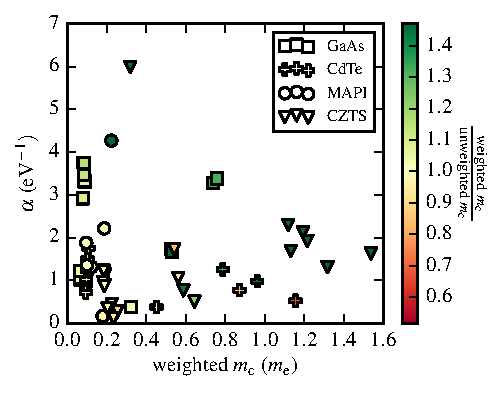
\includegraphics[width=0.6\textwidth]{./figures/ch4/mass_alpha_ratio.pdf}
\caption[Band non-parabolicity vs effective mass]{\label{mass_alpha_ratio}$\alpha$ (a measure of band non-parabolicity) is plotted against the curvature effective mass $m_\text{c}$. The colour scale represents the ratio between the masses calculated using a Fermi--Dirac weighting and no weighting. We use the data from Table\ \ref{masstable}, plus two extra valence bands in \ce{Cu2ZnSnS4} which are higher in binding energy due to crystal field splitting. All results use the HSE06 functional with spin-orbit coupling.} 
\end{figure}

The weighted least-squares fit is an improvement over previous calculation methods as it is less sensitive to the sampling density used, and gives a physically-intuitive energy range to fit over. 
It avoids polynomial fitting to an arbitrarily chosen energy range. 
For light, parabolic bands we find that the three different methods we compare lead to comparable results.
The difference between the calculation methods is greatest for bands with low dispersion and high non-parabolicity.

\subsection{Deviations from the expected effective mass trend}

There are two deviations from the expected trends in the effective mass results, Table \ref{largetable}. 
Firstly; in Table \ref{largetable} we see that the GaAs unweighted heavy-hole mass along [111] is smaller than for [100], while this is the opposite for the other methods. To explain this we should consider the non-parabolicity of the GaAs heavy-hole in the [111] direction (denoted $m_{hh}$[111]). The alpha for parameter for $m_{hh}$[111] is $1.7\,\mathrm{eV}^{-1}$ and so we expect the weighted effective mass to be heavier than the unweighted effective mass (as it samples the heavier states away from band edge). This is confirmed (weighted: $0.53\,m_e$, unweighted: $0.25\,m_e$). Compare this to the alpha parameter for $m_{hh}$[100] which is $0.38\,\mathrm{eV}^{-1}$. This alpha parameter indicates that the dispersion in the [100] direction is near parabolic, and so we would expect the weighted and unweighted masses to be similar. This is also confirmed in our calculations (weighted: $0.32\,m_e$, unweighted: $0.31\,m_e$).
This means that at band edge $m_{hh}\mathrm{[111]} < m_{hh}\mathrm{[100]}$ but due to high non-parabolicity in the [111] direction, when we use our weighted approach and take into account eigenstates away from band edge, $m_{hh}\mathrm{[111]} > m_{hh}\mathrm{[100]}$.

Secondly; in Table \ref{largetable} we see that the CdTe $m_{hh}$[111] is larger for the unweighted method than for the weighted method. This is not the trend seen for the other materials, nor is it the trend we would expect, as the weighted method samples eigenstates away from band edge where the band (approximated by the Kane dispersion) flattens.
This deviation indicates that the Kane dispersion is not an accurate approximation for the CdTe heavy hole band in the [111] direction. The Kane dispersion we use to describe the electronic bands is accurate when the transport effective mass grows linearly with the electron eigenstate energy (Equation \ref{kanemass} of main text). This is the case for most band dispersions in this study, however a plot of transport mass against energy for the CdTe heavy hole in the [111] direction shows that the transport mass is almost constant at small energies - this corresponds to a flattening at the top of the valence band (Figure \ref{mt_E_hh}). We compare this to the light hole in the [111] direction, which shows a linear relationship between transport mass and energy (Figure \ref{mt_E_lh}). This light hole has a weighted mass heavier than the unweighted mass (Table \ref{largetable}), as would be expected for an electronic band described by the Kane dispersion.
%%%% GET RIGHT EQN NUM ABOVE

\begin{figure}[htb] \centering
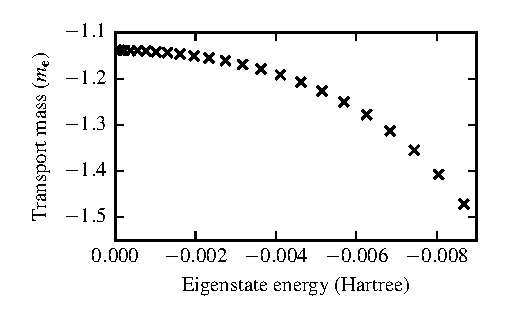
\includegraphics[width=0.6\textwidth]{./figures/ch4/mt_E_hh.pdf}
\caption[Transport effective mass of the CdTe heavy hole]{\label{mt_E_hh}Transport effective mass of the CdTe heavy hole band in the [111] direction, as a function of eigenstate energy (referenced from the valence band maximum).}
\end{figure}

\begin{figure}[htb] \centering
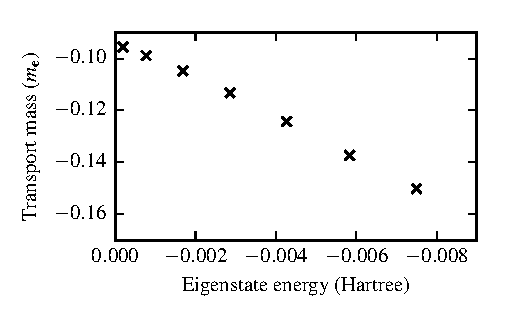
\includegraphics[width=0.6\textwidth]{./figures/ch4/mt_E_lh.pdf}
\caption[Transport effective mass of the CdTe light hole]{\label{mt_E_lh}Transport effective mass of the CdTe light hole band in the [111] direction, as a function of eigenstate energy (referenced from the valence band maximum).}
\end{figure}

\subsection{Sensitivity of the curvature effective mass to the level of theory}

In the previous section we considered the sensitivity of the curvature effective mass to the numerical method used.
In this section we consider how sensitive the curvature effective mass is to the exchange-correlation functional (LDA/GGA/HSE06) and spin-orbit coupling.
We plot the weighted curvature effective mass against the bandgap, at different levels of theory, in Figure\ \ref{m*_bandgap_plot}. 
For CZTS, CdTe and GaAs we find that the local (LDA) and semilocal (GGA) approximations for the exchange energy underestimate the bandgap whereas HSE06 provides a better description. This agrees with previous work.\autocite{Deak2010,Heyd2003}
MAPI has an experimental bandgap of $1.53\,\mathrm{eV}$,\autocite{Liu2015} which, due to a cancellation of errors, is in good agreement with the value calculated using PBEsol with no spin-orbit coupling. 

Tight binding theory states that the effective mass is inversely proportional to the coupling strength between the valence and conduction bands.\autocite{Kittel2005} 
This agrees with the positive correlation between the bandgap and the effective mass shown in Figure\ \ref{m*_bandgap_plot}.
For CZTS, CdTe and GaAs, the effective mass calculated with the HSE06 functional gives the best agreement with experimental data, as has been found previously.\autocite{Kim2010} 
The electron effective mass in CZTS is particularly sensitive to the exchange-correlation energy; the value calculated using the HSE06 functional ($0.19\,m_{\text{e}}$) is over three times that calculated using the LDA or GGA functional ($0.06\,m_\text{e}$).

Spin-orbit coupling has a negligible impact of the effective mass values calculated for CdTe, GaAs and CZTS.
In contrast, spin-orbit coupling does have a large influence on the effective mass values calculated for MAPI, due to the atomic weight of lead. 
A reduced effective mass $((m^{*-1}_{\text{e}}+m^{*-1}_{\text{h}})^{-1})$ of 0.104 has been reported experimentally,\autocite{Miyata2015} for MAPI.
This is equal to the reduced mass calculated in the [100] direction using the hybrid HSE06 functional with spin-orbit coupling ($m^*_{\text{h}}=0.23$, $m^*_{\text{e}}=0.19$). 
Without spin-orbit coupling the effective masses are signficantly overestimated. 

\begin{figure}[tb] \centering
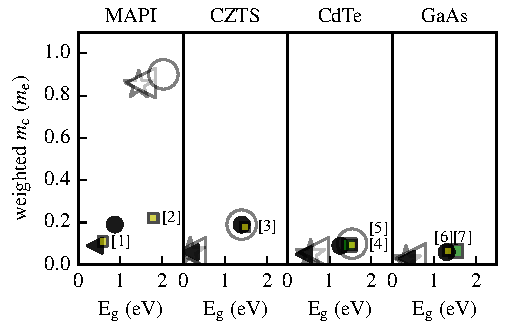
\includegraphics[width=0.6\textwidth]{./figures/ch4/m__bandgap_plot.pdf}
\caption[Effective mass vs bandgap]{\label{m*_bandgap_plot}The effective mass of conduction band electrons in the [100] direction is plotted against the bandgap and Fermi level (referenced to the CBM). The effective mass is calculated using a weighted quadratic least-squares fit as outlined in Section \ref{ch4:methods}. We use filled shapes to denote a calculation with spin-orbit coupling. We use stars, triangles and circles to denote the use of the LDA, PBEsol and HSE06 exchange-correlation functionals respectively. Yellow squares denote results from other computational studies: [1] DFT+SoC\autocite{Filip2015} [2] GW\autocite{Filip2015} [3] DFT+SoC\autocite{Liu2012} [5] GW\autocite{Deguchi2016}  [6] 30-band $k\cdot p$ method.\autocite{Richard2004} Green squares denote results from experimental studies [4] (obscured by [5]) cyclotron resonance\autocite{Madelung2004} [7] cyclotron resonance.\autocite{Madelung2004}}
\end{figure}

\subsection{Sensitivity of the Kane dispersion parameters to the level of theory}

Until this point we have approximated the bandstructures with a parabola, and the effective mass could be described with a single parameter.
We will now approximate the bandstructures with the Kane quasi-linear dispersion. As a result, the effective mass will have two parameters; the effective mass at the band edge and the $\alpha$ parameter (Eqn.\ \ref{kanemass}).

We find that $\alpha$ is inversely correlated with the band gap of the material for all materials in this study (Figure\ \ref{alpha_bandgap_plot}). 
In CZTS, for example, we find that the CB is highly non-parabolic ($\alpha\approx3.5\,\textrm{eV}^{-1}$) at lower levels of theory (LDA/GGA).
However, when we use a hybrid functional the bandgap is increased and the CB becomes more parabolic ($\alpha\approx1\,\textrm{eV}^{-1}$).
We attribute this to the $k\cdot p$ interaction between the conduction and valence bands,\autocite{Kane1957} which makes non-parabolicity particularly pronounced in narrow bandgap semiconductors such as GaAs.\autocite{Szmyd1990}

\begin{figure}[tb] \centering
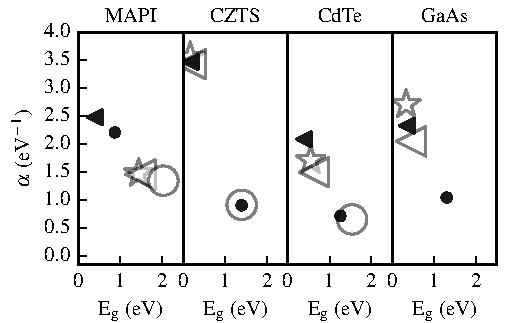
\includegraphics[width=0.6\textwidth]{./figures/ch4/alpha_bandgap_plot.pdf}
\caption[Band non-parabolicity vs bandgap]{\label{alpha_bandgap_plot}$\alpha$ (a measure of band non-parabolicity) is plotted against bandgap at various levels of theory. $\alpha$ is calculated for the CB in the [100] direction. We use filled shapes to denote a calculation with spin-orbit coupling. We use stars, triangles and circles to denote the use of the LDA, PBEsol and HSE06 exchange-correlation functionals, respectively. }
\end{figure}

The non-parabolicity of bands in CZTS\autocite{Ito2015} and MAPI\autocite{Brivio2014,Mosconi2017} has been previously attributed to the spin-orbit interaction. 
We find that, for CZTS, non-parabolicity in the CB is due to the change in bandgap; spin-orbit coupling has only small effect (Figure\ \ref{alpha_SoC}). 
Spin-orbit coupling has a larger effect on the non-parabolicity of the CZTS VB, which has an $\alpha$ value of $3.96\,\textrm{eV}^{-1}$ when calculated with spin-orbit coupling and $1.47\,\textrm{eV}^{-1}$ when calculated without. 
For MAPI, there is increased non-parabolicity in both the VB and CB when spin-orbit effects are considered. 

\begin{figure}[tb] \centering
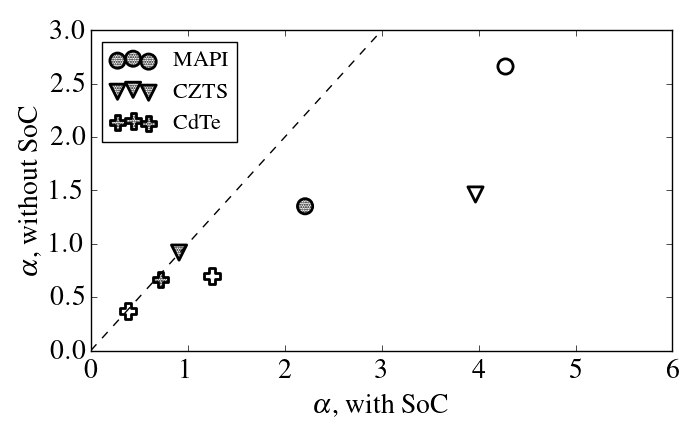
\includegraphics[width=0.6\textwidth]{./figures/ch4/alpha_SoC.png}
\caption[Band non-parabolicity and spin-orbit coupling]{\label{alpha_SoC}$\alpha$ (a measure of band non-parabolicity, eV$^{-1}$) in the [100] direction, calculated with and without spin-orbit coupling. We use hatched shapes to denote an electron in the conduction band, and empty shapes to denote a hole in the valence band. Note the scale; the dashed line indicates where the values would lie if spin-orbit coupling had no influence on the value of $\alpha$. The hybrid HSE06 exchange-correlation functional was used for all calculations. }
\end{figure}

To accurately calculate effective mass parameters, it is important to reproduce the correct band gap.
For CdTe, GaAs and CZTS this is achieved through use of the HSE06 functional.
Without this, the effective mass is under-estimated and band non-parabolicity is over-estimated.
CZTS is particularly sensitive to the exchange-correlation functional used.
The story is different for MAPI: 
reproducing the correct bandgap does not necessarily lead to accurate effective mass values.
Instead, to calculate accurate effective mass values and capture the full extent of band non-parabolicity, we must account for spin-orbit effects.

\subsection{Consequences of non-parabolicity on the optical and transport properties of MAPI}

The effective mass is commonly calculated and compared across materials because it can be used to model differences in various optical and transport properties.
This also means that the effective mass can be inferred from a number of different measurements, which can lead to discrepancies.
For non-parabolic bandstructures, \textit{e.g.} MAPI, these values will also vary with temperature and carrier concentration.
In interpreting the photophysical behaviour of MAPI a range of effective mass values can be found in the literature, from $0.09\,m_{\text{e}}$--$0.30\,m_{\text{e}}$).\autocite{Miyata2015,Tanaka2003,Hirasawa1994,Yang2015,Manser2014,Price2015}
We will focus briefly on the results from transient absorption spectroscopy (TAS).
Manser \textit{et al.} calculated the Burstein--Moss shift in MAPI up to a carrier concentration of $1.5 \times 10^{19}\,\mathrm{cm}^{-1}$.\autocite{Manser2014} Assuming a parabolic band dispersion, they calculated an effective mass at band edge of $0.3\,m_{\text{e}}$.
Yang \textit{et al.} found that a parabolic effective mass value of $0.23\,m_{\text{e}}$ reproduced TAS carrier concentration data.\autocite{Yang2015} Their model requires a shift in energy due to `band gap renormalisation', a concept that incorporates multiple physical phenomena, but that can be partially attributed to band non-parabolicity.\autocite{Walsh2008}
Price \textit{et al.} have developed a model which includes photoinduced changes to the refractive index.\autocite{Price2015} This gives a value of $0.14\,m_{\text{e}}$ for the reduced effective mass, assuming a parabolic dispersion, which is in line with results from magneto-absorption experiments\autocite{Miyata2015,Tanaka2003,Hirasawa1994} and theory.\autocite{Brivio2014,Umari2014} 
The error bar in this value, $0.04\,m_{\text{e}}$, is significant and may be attributed to an effective mass which varies with carrier concentration.

In this section we will quantify the extent to which non-parabolicity impacts upon the Burstein--Moss bandgap shift, optical effective mass, and polaron mobility.
To do so, we assume a Kane quasi-linear dispersion and predict, for MAPI, how these observables will vary as a function of carrier concentration.

\subsubsection{Burstein--Moss bandgap shift}

A consequence of the Pauli exlusion principle is that at a particular carrier concentration the Fermi level is pushed into the conduction (or valence) band. 
This band filling leads to the experimentally observable Burstein--Moss shift where the optical bandgap of the material is increased.
The magnitude of the Burstein--Moss shift is given by 
\begin{equation} \label{parabolic_shift}
\Delta_{\text{BM}} =\frac{\hbar^2}{2m^*}(3\pi^2n_{\text{e}})^{\frac{2}{3}},
\end{equation}
where $m^*$ is the reduced effective mass and $(3\pi^2n_{\text{e}})^{2/3}$ is the Fermi wavevector up to which all states are occupied under the free electron model. 
It is most commonly considered in the context of degenerately doped semiconductors; here we consider photo-excited carriers in an undoped material.

The insulator-metal transition marks the point at which a semiconductor becomes degenerate and it is above this point that the Burstein--Moss shift occurs.
Manser \textit{et al.} report an abrupt onset of the Burstein--Moss effect at carrier concentrations of $7.5\!\times\!10^{17}\,\mathrm{cm}^{-3}$.\autocite{Manser2014}
They account for this through trap filling, with traps estimated to be at a density of $2\!\times\!10^{17}\,\mathrm{cm}^{-3}$.
We add to this the density at which the electron polaron wavefunctions overlap, as given by the phenomonological Mott criterion\autocite{Mott1949}, $4\!\times\!10^{17}\,\mathrm{cm}^{-3}$.\autocite{Frost2017} 
This brings us to a total of $6\!\times\!10^{17}\,\mathrm{cm}^{-3}$, which is closer to the reported experimental value. 
This is beyond the operating conditions under one sun, for which we expect a maximum carrier concentration of $\sim10^{16}\,\mathrm{cm}^{-3}$.\autocite{Herz2016} 
However concentrator systems can achieve carrier concentrations of $10^{18}\,\mathrm{cm}^{-3}$ \autocite{Law2014} and will fall into the degenerate regime.
Furthermore, carrier concentrations of up to $10^{19}\,\mathrm{cm}^{-3}$ are reached when exciting with a laser as in photoluminescence and transient absorption spectroscopy measurements,\autocite{Richter2016}
and there has been recent research interest in developing a hybrid halide perovskite lasing material which would require concentrations of up to $10^{21}\,\mathrm{cm}^{-3}$.\autocite{Gao2017}

We assume a parabolic dispersion and use the curvature effective mass to calculate values of the Burstein--Moss shift using Eqn.\ \ref{parabolic_shift}. When we compare our results to the density of states data calculated from DFT, which makes no assumption about the form of the dispersion, we see that the parabolic approximation leads to a large overestimation (Figure\ \ref{burstein_moss_plot}). 
Walsh \textit{et al.}\autocite{Walsh2008} demonstrated that non-parabolicity can cause this discrepancy, as
non-parabolicity increases the density of states, which results in the Fermi level increasing more slowly. 
We account for non-parabolicity by substituting the energy-dependant mass given by Eqn.\ \ref{kanemass} into Eqn.\ \ref{parabolic_shift} and solving self-consistently.
With this amendmant we see good agreement with the density of states data; this demonstrates that the Kane quasi-linear dispersion provides a suitable approximation at high carrier concentrations.

\begin{figure}[tb] \centering
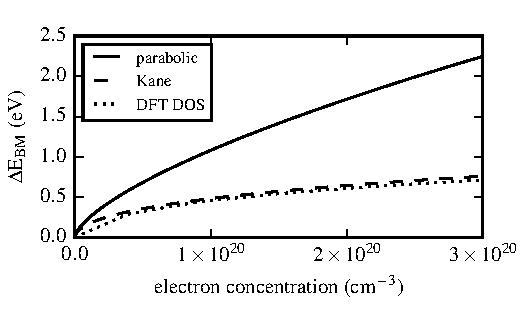
\includegraphics[width=0.6\textwidth]{./figures/ch4/burstein_moss_MAPI_hybrid_SoC.pdf}
\caption[Burstein--Moss band gap shift]{\label{burstein_moss_plot} The Burstein--Moss band gap shift is plotted as a function of carrier concentration. The shift is calculated assuming a parabolic dispersion, Kane quasi-linear dispersion and from a DFT calculated density of states. Beyond this carrier concentration range we begin to fill bands higher in energy (the secondary band in MAPI is calculated to be at $0.78\,\mathrm{eV}$). To average across different directions we use the geometric mean of the effective mass and the arithmetic mean of $\alpha$.}
\end{figure}

\subsubsection{Optical effective mass}

To calculate the effective mass which is measured in optical experiments, we integrate the analytic expression given in Eqn.\ \ref{opt} with $E(k)$ given by the Kane dispersion in Eqn.\ \ref{kane}. 
We set the Fermi level equal to the Burstein--Moss shift, which gives a dependance on carrier concentration. 

\begin{figure}[tb] \centering
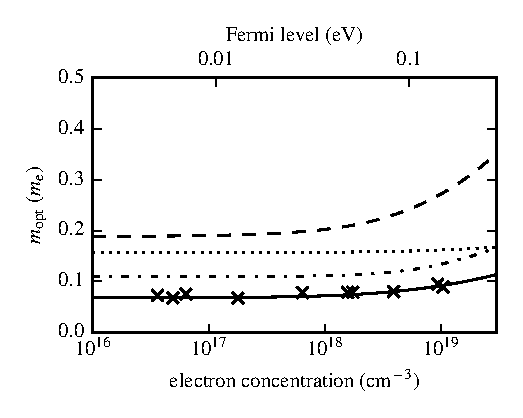
\includegraphics[width=0.6\textwidth]{./figures/ch4/optical_mass_concentration_MAPI.pdf}
\caption[Electron effective mass as a function of carrier concentration]{\label{optical_concentration_plot} The conduction band electron optical effective mass is plotted as a function of carrier concentration. Values for the [100] (dash line), [111] (dot line) and [110] (dash-dot line) directions are given. To validate our results we include results for GaAs (continuous line) and compare this against experimental data (crosses).\autocite{Raymond1979} The Kane quasi-linear dispersion in the [100] direction does not give a good approximation to the DFT-calculated dispersion beyond carrier concentrations of $3\!\times\!10^{19}\,\mathrm{cm}^{-3}$. }
\end{figure}
% also, by chance, the GaAs secondary band at 0.35 eV corresponds to 3E19.

At a concentration of $3\!\times\!10^{19}\,\mathrm{cm}^{-3}$ there is a significant increase in the optical effective mass in the [100] direction, from $0.19\,m_\text{e}$ at the band edge to a value of $0.35\,m_\text{e}$ (Figure\ \ref{optical_concentration_plot}). 
To put this in context, the effective mass values calculated using GW+SoC and DFT+SoC differ by up to only $0.03\,m_\text{e}$.\autocite{Umari2014}
Clearly, at high carrier concentrations, we must account for non-parabolicity to achieve accurate estimates for the optical effective mass.
This result is highly dependant on the non-parabolicity of the bandstructure; we see a negligible increase in the optical effective mass in the [111] direction due to the small value of $\alpha$ in this direction. 

\begin{table*} \centering
\caption[Electron effective mass and polaron mobility at various carrier concentrations]{\label{masstable} The optical effective mass and polaron mobility for a conduction band electron in the [110] direction of \ce{CH3NH3PbI3}. AM1.5 is the global standard solar spectrum for non-concentrator systems.}
\begin{tabular}{p{3.5cm}p{3.5cm}p{3.5cm}p{4cm}}
\toprule
conc. (cm$^{-3}$) & eff. mass $m_\text{opt}$ ($m_\text{e}$) & mobility ($\frac{\text{cm}^2}{\text{Vs}}$) & application \\
\midrule
10$^{15}$ & 0.11 & 158 & solar cell AM1.5\\
10$^{18}$ & 0.11 & 158 & concentrator system \\
10$^{19}$ & 0.13 & 120 & photoluminescence\\
10$^{20}$ & 0.23 & 46 & lasing material \\
\bottomrule
\end{tabular}
\end{table*}


\subsubsection{Polaron mobility} \label{ch4:mobility}

The relationship between the mobility $\mu$, relaxation time $\tau$ and effective mass $m^*$ of a particle with charge $q$ is given by

\begin{equation}
\mu = \frac{q\tau}{m^*}.
\end{equation}

On first inspection it would seem that the mobility must be directly proportional to the inverse of the effective mass. 
However, for a range of scattering processes, the relaxation time is not independant of the effective mass and this will lead to a more complex relationship between effective mass and mobility.
We use a model which considers scattering from polar optical phonon modes,
as this is the process which limits the charge carrier mobility in MAPI at room temperature.\autocite{Wright2016}

We calculate polaron mobility using a recently implemented \textit{ab-initio} method based on a Feynman path integral approach.\autocite{Frost2017b}
The parameters for this model are the effective mass, high- and low-frequency dielectric constants and a characteristic phonon mode.
Here we study the effects of band non-parabolicity by calculating electron polaron mobility as a function of the optical effective mass. 
We justify using the optical effective mass to calculate a transport property with reference to Eqn.\ \ref{opt}.

\begin{figure}[tb] \centering
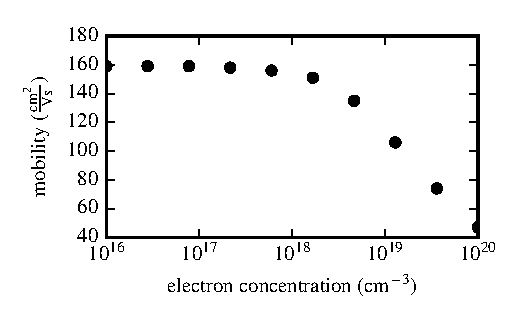
\includegraphics[width=0.6\textwidth]{./figures/ch4/mobility.pdf}
\caption[Polaron mobility as a function of carrier concentration]{\label{mobility_plot} Polaron mobility, limited by optic-mode scattering, is plotted as a function of carrier concentration for a conduction band electron in the [110] direction of \ce{CH3NH3PbI3}. This is calculated using parameters taken from the literature:\autocite{Frost2017b} high-frequency dielectric constant $=4.5$, low-frequency dieletric constant $=24.1$ and characteristic phonon frequency $=2.25\times10^{12}\,\mathrm{cm}^{-1}$.}
\end{figure}

The mobility at a concentration of $10^{20}\,\mathrm{cm}^{-3}$ is $\sim30\%$ of that calculated for low carrier concentrations (Figure\ \ref{mobility_plot} and Table \ref{masstable}).
This significant reduction happens even in the absence of the electron--electron scattering that will be enhanced at higher carrier concentrations,
and agrees with a previous report which states that mobility is particularly sensitive to effective mass.\autocite{Ponce2018} 
%These values provide an upper limit for the polaron mobility, without considering other scattering process (defect--carrier, carrier--carrier) which will depend on carrier concentration and may reduce our estimates .

Our results show that non-parabolicty has a negligible effect on the optical effective mass and mobility of MAPI at concentrations of $\sim10^{18}\,\mathrm{cm}^{-3}$ (Table\ \ref{masstable}).
At a concentration of $1.5\!\times\!10^{18}\,\mathrm{cm}^{-3}$, the Burstein--Moss bandgap shifts we predict using the parabolic and Kane quasi-linear dispersion differ by $0.008\,\text{eV}$.
This is significantly less than the typical energetic disorder at room temperature ($\mathrm{k_\mathrm{B}T}=0.025\,\mathrm{eV}$), and so we predict the parabolic approximation to be sufficient at these carrier concentrations.
At higher concentrations it is important to account for band non-parabolicity to make accurate predictions for the Burstein-Moss bandgap shift, optical effective mass and polaron mobility. 
At a concentration of $10^{20}\,\mathrm{cm}^{-3}$ there is a doubling in the optical effective mass and a three-fold decrease in polaron mobility. 


\section{Summary}

The effective mass plays a central role in the description of several material properties, and is a key parameter when assessing the suitability of materials for use in, for example, photovoltaic applications. 
Several alternative definitions exist for the effective mass, and there are also different ways to numerically calculate these from calculated electronic structure data.

I have introduced a method to calculate the curvature effective mass which uses a physically intuitive energy range given by the Fermi--Dirac distribution. This accounts for the thermal smearing of charge carriers, which is inevitable above $0\,\mathrm{K}$.
I have shown that this method is less sensitive to the sampling density in reciprocal space.

We then moved beyond the parabolic approximation to consider bandstructures described by Kane quasi-linear dispersion.
The $\alpha$ parameter provides a good description of the dispersion away from band edge and could be used as a screening parameter for materials which operate at high carrier concentrations, for example transparent conducting oxides.
It is found that, across the four materials, accurate non-parabolic effective mass values require hybrid functionals as band gap underestimation generally results in artificially high levels of non-parabolicity.
It is also important to account for spin-orbit coupling when describing the non-parabolicity of the valence bands via the $\alpha$ parameter.

Finally, I have considered how non-parabolicity impacts upon optical and transport properties at high carrier concentrations.
For this the lead halide perovskite MAPI was used as a case study, as it was found to be the most highly non-parabolic of the four materials.
It was found that the parabolic approximation severely overestimates the Burstein--Moss shift, 
whilst the Kane quasi-linear dispersion shows good agreement with density of states calculations. 
Using the Burstein--Moss shift as a proxy for the Fermi level, I calculated the change in electron effective mass and mobility as a function of carrier concentration. 
The assumption previously used in the literature---that the effective mass is independant of carrier concentration---is not valid.
At carrier concentrations above $10^{18}\,\mathrm{cm}^{-3}$, non-parabolicity must be built into photophysical models to give accurate values for the effective mass and derived properties.

\textbf{Data Access Statement}

The crystal structures and electronic structure data reported in this chapter, alongside a Jupyter notebook which outlines the key calculation steps, are available 
in an online repository.\autocite{Whalley2018b}
Effective mass values can be calculated using \textsc{effmass} package,\autocite{Whalley2018a} which is outlined in Appendix \ref{app:1-effmass}.
Polaron mobility can be calculated using the \textsc{PolaronMobility.jl} package.\autocite{Frost2018} 

\textbf{Acknowledgements}

This work used the ARCHER UK National Supercomputing Service \\ (http://www.archer.ac.uk) which we have access to via membership of the UK's HEC Materials Chemistry Consortium (funded by EPSRC Grant No. EP/L000202). I am also grateful to the UK Materials and Molecular Modelling Hub for computational resources, which is partially funded by EPSRC Grant No. EP/P020194/1.